\section{Evaluating Visual Object Tracking}
\label{sec:EvaluatingVisualObjectTracking}

In our work, we tackle problems of \Gls{vot}, concretely \gls{mot}, for which there are no established solutions neither for prediction itself nor for its evaluation. The research is practically still ongoing. When it comes to evaluating \gls{mot} performance, even after many years, there is still no consensus how to approach the evaluation and subsequent comparison of multi-object trackers~\cite{bernardin2008clearmot}.

There is one established metric, however, called \gls{clear} \gls{mot} metric~\cite{bernardin2008clearmot} (further referred to as just \gls{clear}), that we will employ to evaluate and quantitatively assess the performance of a \gls{mot} system. The reasons are the following:
\begin{itemize}
    \item This metric is still considered a reasonably effective and intuitive metric to use, despite multiple proposals for improvements~\cite{wen2020uadetrac}.
    \item Numerous works in object tracking, especially tracking of people, report statistics from the \gls{mot} challenges that historically have utilized this metric.
    \item From the engineering perspective, there are standard frameworks (e.g.,~\cite{webpymotmetrics}) that provide evaluation of a custom \gls{mot} tracker inference with a plethora of configurations and additional metrics as a bonus that make peeking into the performance of the tracker a lot easier. For instance, we were particularly interested in additional metrics such as the number of object switches (explained later) etc.
\end{itemize}

Bernardin~\etal{}~\cite{bernardin2008clearmot}, the authors of \gls{clear} discussed above, designed two crucial criteria that performance metrics should meet. Here we present their list in which the first two items are considered primary, whereas the remaining are expected properties of useful metrics, but not necessarily demanded. Therefore, such metrics should:
\begin{enumerate}
    \item allow to assess the tracker's precision regarding how well it is capable of determining the exact object location,
    \item reflect the tracker's ability to track objects consistently, i.e., to correctly trace object trajectories such that one and only one trajectory is established per object,
    \item have as few free parameters as possible,
    \item be clear and easy to interpret while emphasizing intuitive human understanding of the tracking process,
    \item be general enough so that comparison of different types of trackers, e.g. $2$D or $3$D, is possible,
    \item contain expressive values rich in information yet not abundant in quantity.
\end{enumerate}

Considering this, they proposed a systematic approach to evaluating tracker's characteristics. For clarity, we will adopt the notation and nomenclature introduced in~\cite{bernardin2008clearmot}.

Let $t$ denote a time for a specific frame. For each frame $t$, the multi-object tracker produces a set of hypotheses $\cbrackets{h_1, h_2, \dots, h_m}$ for a set of visible objects $\cbrackets{o_1, o_2, \dots, o_n}$. With this in mind, the evaluation procedure can be briefly described in the following pseudocode.

For each time frame $t$:
\begin{enumerate}
    \item establish the best possible correspondence between hypotheses $h_i$ and objects $o_j$, where $i = 1, 2, \dots m$ and $j = 1, 2, \dots, n$,
    \item for each determined correspondence between object and hypothesis:
          \begin{enumerate}
              \item quantify the error in estimation of the object's position,
          \end{enumerate}
    \item perform accumulation of all errors (see \figstr{}~\ref{fig:CLEARHypotheses}) in the found correspondences:
          \begin{enumerate}
              \item count all false negatives (misses), i.e., objects for which there was no hypothesis,
                    item count all false positives, i.e., hypotheses for which there was no object,
                    item count mismatch errors (swaps of object IDs), i.e., situations in which the hypothesis for a given object changed compared to the previous frame.
          \end{enumerate}
\end{enumerate}

% ------------------------------------------------------------------------------
\begin{figure}[t]
    \centerline{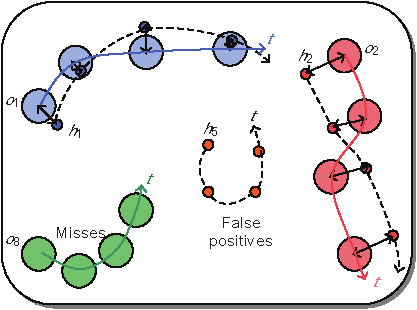
\includegraphics[width=0.55\linewidth]{figures/theoretical_foundations/clear_hypotheses_status.pdf}}
    \caption[\gls{clear} hypotheses]{With a demonstration of a correct tracker inference at the top, the \gls{clear} \gls{mot} metric distinguishes between three fundamental types of errors, misses (false negatives), false positives and ID switches, shown in this order respectively. \externalsrc{\cite{bernardin2008clearmot}}}
    \label{fig:CLEARHypotheses}
\end{figure}
% ------------------------------------------------------------------------------

% ##############################################################################
\subsection{Establishing Correspondences}

The correspondence between a hypothesis $h_i$ and an object $o_j$ should not be made unless their distance (denoted as $d_{i,j}$) is within a specific threshold $T$. The measure of distance has to be defined for each task, but the \gls{iou} distance or Euclidean distance of \gls{bbox} centroids are most commonly used. From now on, we define object-hypothesis correspondence to be valid as long as $d_{i,j} < T$.

The value of $T$ is critical and greatly influences the outcome. Evaluating tracking performance bears the burden of having parameters that are difficult to generalize and the process of setting their values is often accompanied with experimentation. For example, conceptually speaking, there is by all means a boundary (the threshold $T$) beyond which we can no longer speak of an error in position estimation, but rather we could claim that the tracker has drifted away and is tracking a completely different object. With that being said, the exact value of this boundary is up for a discussion.

% ##############################################################################
\subsection{Tracking Consistency}

In order to properly examine the tracker in terms of how consistent it is at tracking objects, one has to detect conflicting predictions for the given object over time. We acknowledge that there may be numerous approaches to this problem. Bernardin~\etal{}~\cite{bernardin2008clearmot} remarked that such procedures somehow need to decide what the ``best'' mapping is. For instance, assuming an object $o_j$ and a hypothesis $h_i$, the ``optimal'' matching may be based on the initial correspondence made for $o_j$ or the most frequent correspondence made throughout the whole sequence. If any violation is encountered, it is then treated as a discrepancy and thus counted as error.

However, there are several issues with such approaches. Consider scenarios depicted in \figstr{}~\ref{fig:SeqLevelMostCommonCorrespondenceProb}. The authors raised their concerns regarding the objectivity of such evaluation and proposed a slightly different method. They only count mismatch errors once at the time frame where the change occurrs, and consider the remaining intermediate correspondences as correct. We agree with such objection, since local discrepancy in object-hypothesis correspondence may indicate just a temporary drift the tracker, whereas its ability to preserve the object's identity does not necessarily have to be so poor as the original metric would display.

Let $M_t = \cbrackets{\rbrackets{h_i, o_j}}$ be the set of mappings made up to time $t$, such that $M_0 = \cbrackets{\cdot}$. Once a new correspondence is made at the next step at time $t + 1$ between the hypothesis $h_k$ and the object $io_j$ that conflicts the already established identity by the pair $\rbrackets{h_i, o_j}$ in $M_t$, this contradition is then counted as a mismatch error and $\rbrackets{h_i, o_j}$ is replaced by $\rbrackets{h_k, o_j}$ in $M_{t + 1}$. Consequently, papping that is constructed this way enhances decision-making when facing multiple competing hypotheses for the same object. The implicit assumption is that the previously assigned hypothesis is more likely to be correct that the new one, even if the distance metric alone would indicate otherwise (see \figstr{}~\ref{fig:ObjectHypothesisReInit} for illustration).

% ------------------------------------------------------------------------------
\begin{figure}[t]
    \centerline{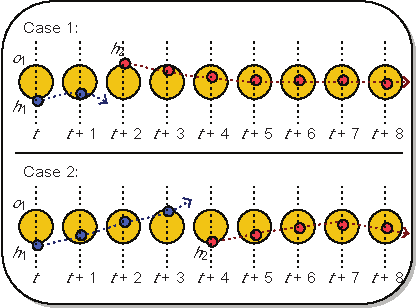
\includegraphics[width=0.5\linewidth]{figures/theoretical_foundations/seq_based_correspondence_issues.pdf}}
    \caption[Sequence-based correspondence mismatches]{This figure illustrates the inherent ``unfairness'' when relying on sequence-level ``best'' object-hypothesis mapping induced by the most frequent correspondence. As shown in the case $1$, the correct hypothesis is the $h_2$, and thus only $2$ errors are incurred for the first mismatch. The case $2$ is practically identical, the $h_2$ also represents the most common assignment. However, $4$ errors are accumulated for the alleged mismatch for $h_1$. \externalsrc{\cite{bernardin2008clearmot}}}
    \label{fig:SeqLevelMostCommonCorrespondenceProb}
\end{figure}
% ------------------------------------------------------------------------------

% ------------------------------------------------------------------------------
\begin{figure}[t]
    \centerline{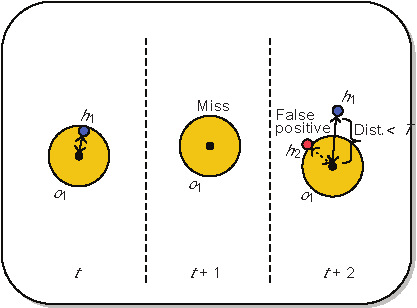
\includegraphics[width=0.5\linewidth]{figures/theoretical_foundations/object_hypothesis_reinit.pdf}}
    \caption[Object-hypothesis re-initialization]{Demonstration of a track reinitialization. At time $t$, the identity of the object $o_1$ is accounted for by the hypothesis $h_1$. At time $t + 1$, the object disappears and the track is temporarily lost. At time $t + 2$, the tracker is responsible for reinstantiating the object identity. During evaluation, the underlying assumption is that the previous hypothesis should be the correct one, even if the new hypothesis is closer according to the used distance function. \externalsrc{\cite{bernardin2008clearmot}}}
    \label{fig:ObjectHypothesisReInit}
\end{figure}
% ------------------------------------------------------------------------------

% ##############################################################################
\subsection{Mapping Procedure}

In what follows, we will describe a recipe for the mapping procedure based on the previously discussed foundations.

Let $M_0 = \cbrackets{\cdot}$. For each time frame $t$:
\begin{enumerate}
    \item Verify if every mapping in $\rbrackets{h_i, o_j}$ in $M_{t - 1}$ is still valid. Such pair is deemed valid as long as the hypothesis $h_i$ exists at time $t$, the object $o_j$ is still visible while the distance between the two does not exceed $T$. If these conditions hold, establish a correspondence.
    \item If there are objects for which no correspondence has been made so far, then a suitable matching hypothesis is searched for. This step involves one-to-one matching for pairs the distance of which does not exceed the threshold $T$. The matching procedure is formulated as minimum cost assignment problem and Munkres's algorithm~\cite{munkres1957assignment} can be adopted. In case there happens to be a correspondence that contradicts a mapping $\sbrackets{h_i, o_j}$ as part of $M_{t - 1}$, then replace the previous pair $\sbrackets{h_i, o_j}$ with $\sbrackets{h_k, o_j}$ and treat such an occurrence as a mismatch error. For simplicity, let $mme_t$ be the number of the mismatch errors for the frame $t$.
    \item The two previous steps guaratee that a complete set of matching pairs has been generated for the current time $t$. At this point, we may start calculating values that will be utilized later on for computing the final metrics. So, let $c_t$ be the number of matches found for time $t$. For each such match, compute the distance (once again, up to the designer's choice) between the object $o_j$ and the corresponding hypothesis, denoted by $d_{ti}$.
    \item Every hypothesis that is not part of any pair up to this point is reckoned as false positive. Likewise, all the remaining objects are marked as misses, i.e., false negatives. Thus, let $fp_t$ and $m_t$ be the number of false positives and misses, respectively. For sakes of computation, let us define $g_t$ as the number of ground-truth objects visible at time $t$.
\end{enumerate}

Please note that no mismatch errors can occurr at the initial frame as the set of mappings $M_0$ is empty and therefore all correspondences are treated as initializations.

% ##############################################################################
\subsection{Performance Metrics}

In light of the previously described procedure and introduced notation, here we present the two most relevant performance metrics by which the tracking performance can be intuitively expressed using two quantities, namely the ``tracking precision'' and ``tracking accuracy''. Even though it could be argued whether such expression is sufficient.

In general terms, the role of tracking precision is to measure the alignment between the predicted object position (e.g., its \gls{bbox}) and the groud-truth position only for the positive sample. With that being said, precision is not influenced by the ability (or lack thereof) of the tracker to detect objects properly. It is designed to evaluate the suitability of the delineation of the object \gls{bbox} the detection of which was correct in the first place. The \gls{motp} metric can thus be defined as
\begin{equation}
    \label{eq:MOTPMetric}
    \text{MOTP} = \frac{\sum_{\forall t} \sum_{\forall i} d_{ti}}{\sum_{\forall t} c_t},
\end{equation}
\eqstr{}~\ref{eq:MOTPMetric} represents the total error in the estimated position for the pairs where the object-hypothesis relationship was correctly determined averaged over the total number of such matches made. As stated above, it gauges the ability of the tracker to estimate precise object positions regardless of its capability of recognizing them or keeping their trajectories consistent.

Conversely, the accuracy metric attempts to reflect the number of mistakes the tracker made in terms of misses, false positives, object mismatches, failures to recover already established tracks, and so forth. Given this description, the \gls{mota} metric can be expressed as
\begin{equation}
    \label{eq:MOTAMetric}
    \text{MOTA} = 1 - \frac{\sum_{\forall t} \rbrackets{m_t + fp_t + mme_t}}{\sum_{\forall t} g_t},
\end{equation}
the possible values of which lie within the interval $\sbrackets{-\infty, 1}$. For example, if a tracker produces a lot of false positives, the value in the sum may actually exceed one, and therefore, the final metric would be negative.

We would like to emphasize that the errors have to be first summed up across all the frames before computing the ratios rather than evaluating the ratio locally. Independent computation of the given ratios (in both equations~\ref{eq:MOTPMetric}~and~\ref{eq:MOTAMetric}) would lead to non-intuitive outcome (see \figstr{}~\ref{fig:LocalGlobalRatioEval} for details).

% ------------------------------------------------------------------------------
\begin{figure}[t]
    \centerline{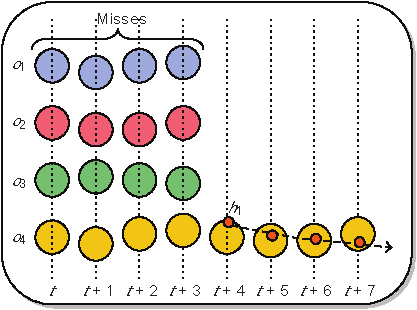
\includegraphics[width=0.6\linewidth]{figures/theoretical_foundations/local_vs_global_ratio_evaluation.pdf}}
    \caption[Local vs. global ratio evaluation]{Computing of error ratios needs to be performed on a global level, rather than on a local, frame level. Assume a sequence consisting of $8$ frames. Moreover, assume that objects $o_1, \dots, o_4$ are visible on the frames from $t_1$ to $t_4$, but none of them is being tracked. The situation changes at frame $t_4$ where only the object $o_4$ is being tracked properly by the hypothesis $h_1$. As a result, in frames $t_1, \dots, t_4$, the resulting miss rate is $100\%$, whereas in frames $t_5, \dots, t_8$ it is exactly $0\%$. Applying arithmetic average to these values yields a global miss rate of $\frac{1}{8} \rbrackets{4 \cdot 100 + 4 \cdot 0} = \frac{1}{2}$, or, $50\%$. Conversely, performing summation prior to quantifying the final global ratio produces far more intuitive result of $16$ out of $20$ misses, or the miss rate of $80\%$. \externalsrc{\cite{bernardin2008clearmot}}}
    \label{fig:LocalGlobalRatioEval}
\end{figure}
% ------------------------------------------------------------------------------
